\documentclass[10pt,a4paper]{article}
\usepackage[utf8]{inputenc}
\usepackage{amsmath}
\usepackage{amsfonts}
\usepackage{amssymb}
\usepackage{graphicx}
\title{Infrastructure du réseau UCL}
\begin{document}
\maketitle
\section{InterMapper Devices}
Au niveau de la carte on a 6 \textbf{routeurs de quartier} avec leur nom qui commence par \texttt{CT}. Il s'agit des routeurs Pythagore, Halles, Michotte, SH1C, Stevin et CTLew. Ils ne s'occupent \textbf{que du routage}.\\
CTLew c'est le routeur de Wolluwé.\\
Au niveau de la connexion, la connexion principale Belnet est à 10Gb/sec et la connexion de secours est à 3Gb/s mais n'est pas utilisée.\\
Les routeurs \textbf{CTTier2} et \textbf{CTAquarium} sont les \textbf{datacentres}. Ils contiennent les Radius et les LDAP.\\\\
On a également des \textbf{commutateurs} dans chaque batiment (représentés sur la carte par des chiffres par exemple 01-07-002). Chaque commutateur possède 48 ports et on ils sont parfois reliés entre eux).\\\\

Concrètement, dans chaque batiment il y a des prises qui sont reliées à des points de \textbf{concentration}. Ces points de concentrations contiennent des commutaturs qui peuvent être reliés à un commutateur de batiment qui lui est relié au routeur.
\begin{figure}[h!]
   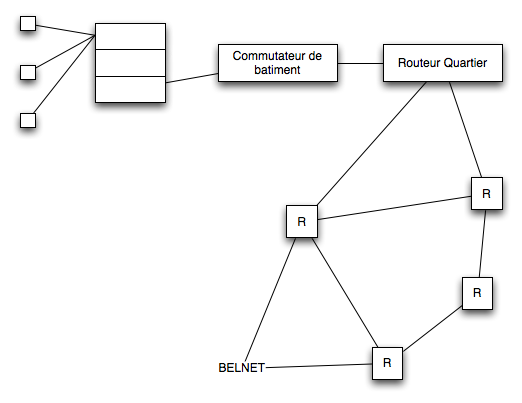
\includegraphics[scale=0.5]{images/infrastructure/infrastructure.png}
\end{figure}
Le réseau \textbf{n'est pas en full mesh !}\\

\textbf{WiSM} représente tous les controlleurs wifi.\\
\textbf{WiSM1} = anciens controllers (4)\\
\textbf{WiSM2} = nouveaux controllers (2)

\section{Topologie réseau wifi}
\begin{figure}[h!]
   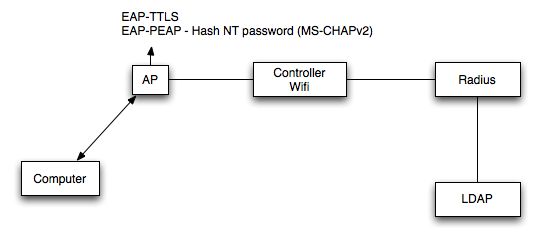
\includegraphics[scale=0.7]{images/infrastructure/topologie.png}
\end{figure}

Les \textbf{AP} contiennent la clé WPA,... mais elles ne connaissent pas grand chose. Elles comprennent l'EAP mais ne savent pas le déchiffrer.\\
Si on veut s'authentifier, l'AP sait qu'on fait du 802.1x donc il sait qu'il doit demander des choses au client.\\
L'AP comprend l'EAP et le transmet au controller.\\
Le controller parle au Radius et EAP est décrypté par le Radius.\\\\
On a 2 tunnels: un pour l'EAP et un pour le TTLS ou PEAP\\\\

Au niveau du \textbf{materiel}, il y 2 Radius et il reste 40 bornes sur le WiSM1. En tout il y a environ 350 bornes en tout sur LLN.\\\\

Au niveau du \textbf{Radius}, si on a une adresse provenant de l'univeristé de Namur et qu'on veut se connecter sur Eduroam à LLN, le Radius ne connait pas l'adresse @namur.be. Il va donc l'envoyer au Radius de \textbf{Belnet}. Belnet voit qu'il s'agit d'une adresse de Namur donc il l'envoie au Radius de \textbf{Namur} qui va renvoyer "OK pour la connexion" à Belnet qui va la renvoyer au Radius de l'UCL.\\
Si on passe par \textbf{ethernet}, le commutateur est directement connecté au Radius\\\\

Le \textbf{Catalyst 6509} contient 6 parties :
\begin{itemize}
\item Un controller (processeur)
\item Une carte 1Gb en fibre optique
\item Une carte 1Gb en cuivre
\item Une carte 100Mb en fibre optique
\item WiSM
\item Firewall
\end{itemize}

\section{Adresses IP}
\begin{itemize}
\item \texttt{127.0.0.1}: Uniquement utilisé par les clients TTLS parce qu'il y a un double tunnel (un 2ème tunnel à l'intérieur de lui même).
\item \texttt{10.253.12.3,4}: Controller Wolluwé
\item \texttt{192...171,178,181,182}: Les 4 WiSM1
\item \texttt{192...169,170}: Les 2 WiSM2
\item \texttt{130.104.1.11}: Machine qui fait du monitoring (wificheck)
\item \texttt{130.104.10.134}: Machine de Dominique Margot
\item \texttt{172.31.15.6}: 802.1x par cable
\item \texttt{193.190.198.33,59}: Radius Belnet
\end{itemize}

\section{DHCP}
Le lease time est de 900secondes par défaut et peut monter à 1800sec

\end{document}
